\hypertarget{Line_8h}{
\section{/PIWO/Program/gui/Line.h File Reference}
\label{Line_8h}\index{/PIWO/Program/gui/Line.h@{/PIWO/Program/gui/Line.h}}
}
{\tt \#include $<$SysUtils.hpp$>$}\par
{\tt \#include $<$Classes.hpp$>$}\par
{\tt \#include $<$Controls.hpp$>$}\par


Include dependency graph for Line.h:\nopagebreak
\begin{figure}[H]
\begin{center}
\leavevmode
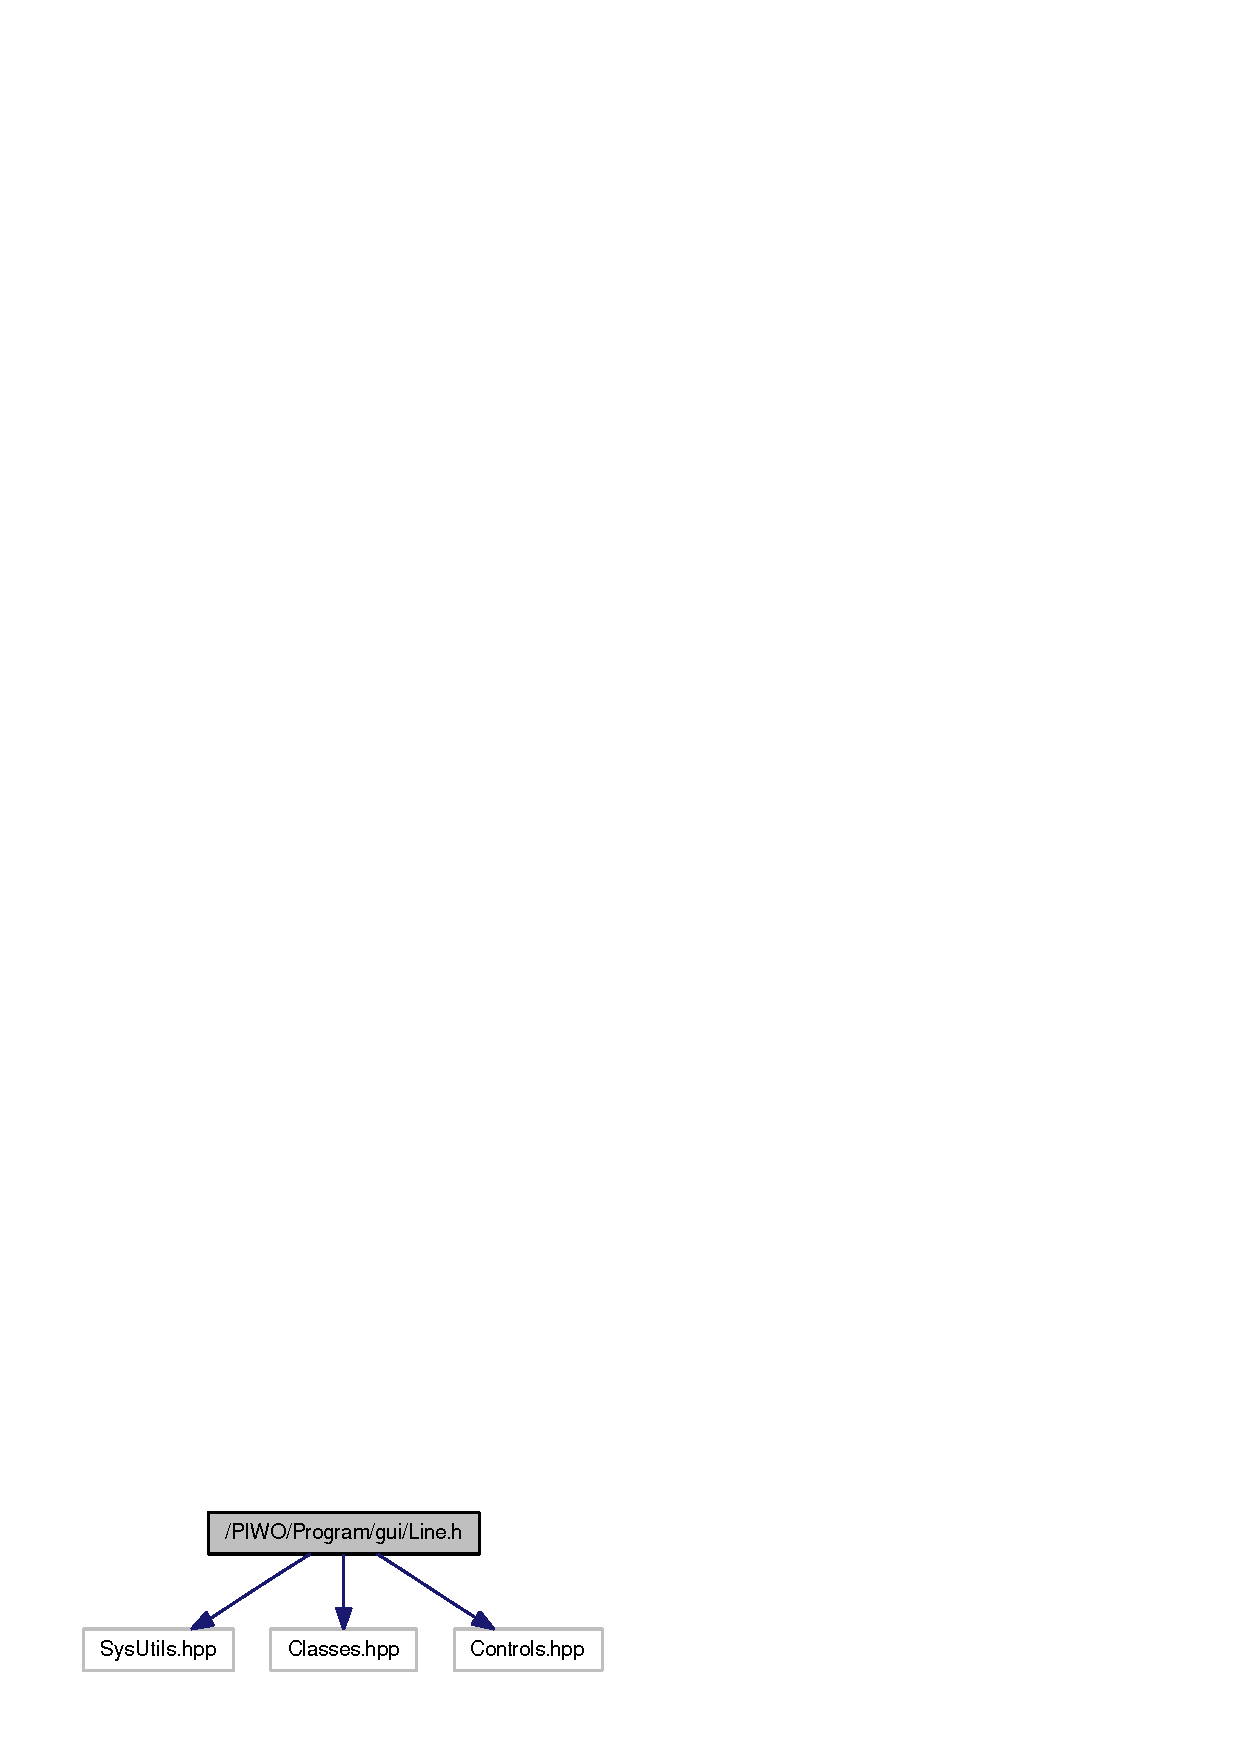
\includegraphics[width=146pt]{Line_8h__incl}
\end{center}
\end{figure}


This graph shows which files directly or indirectly include this file:\nopagebreak
\begin{figure}[H]
\begin{center}
\leavevmode
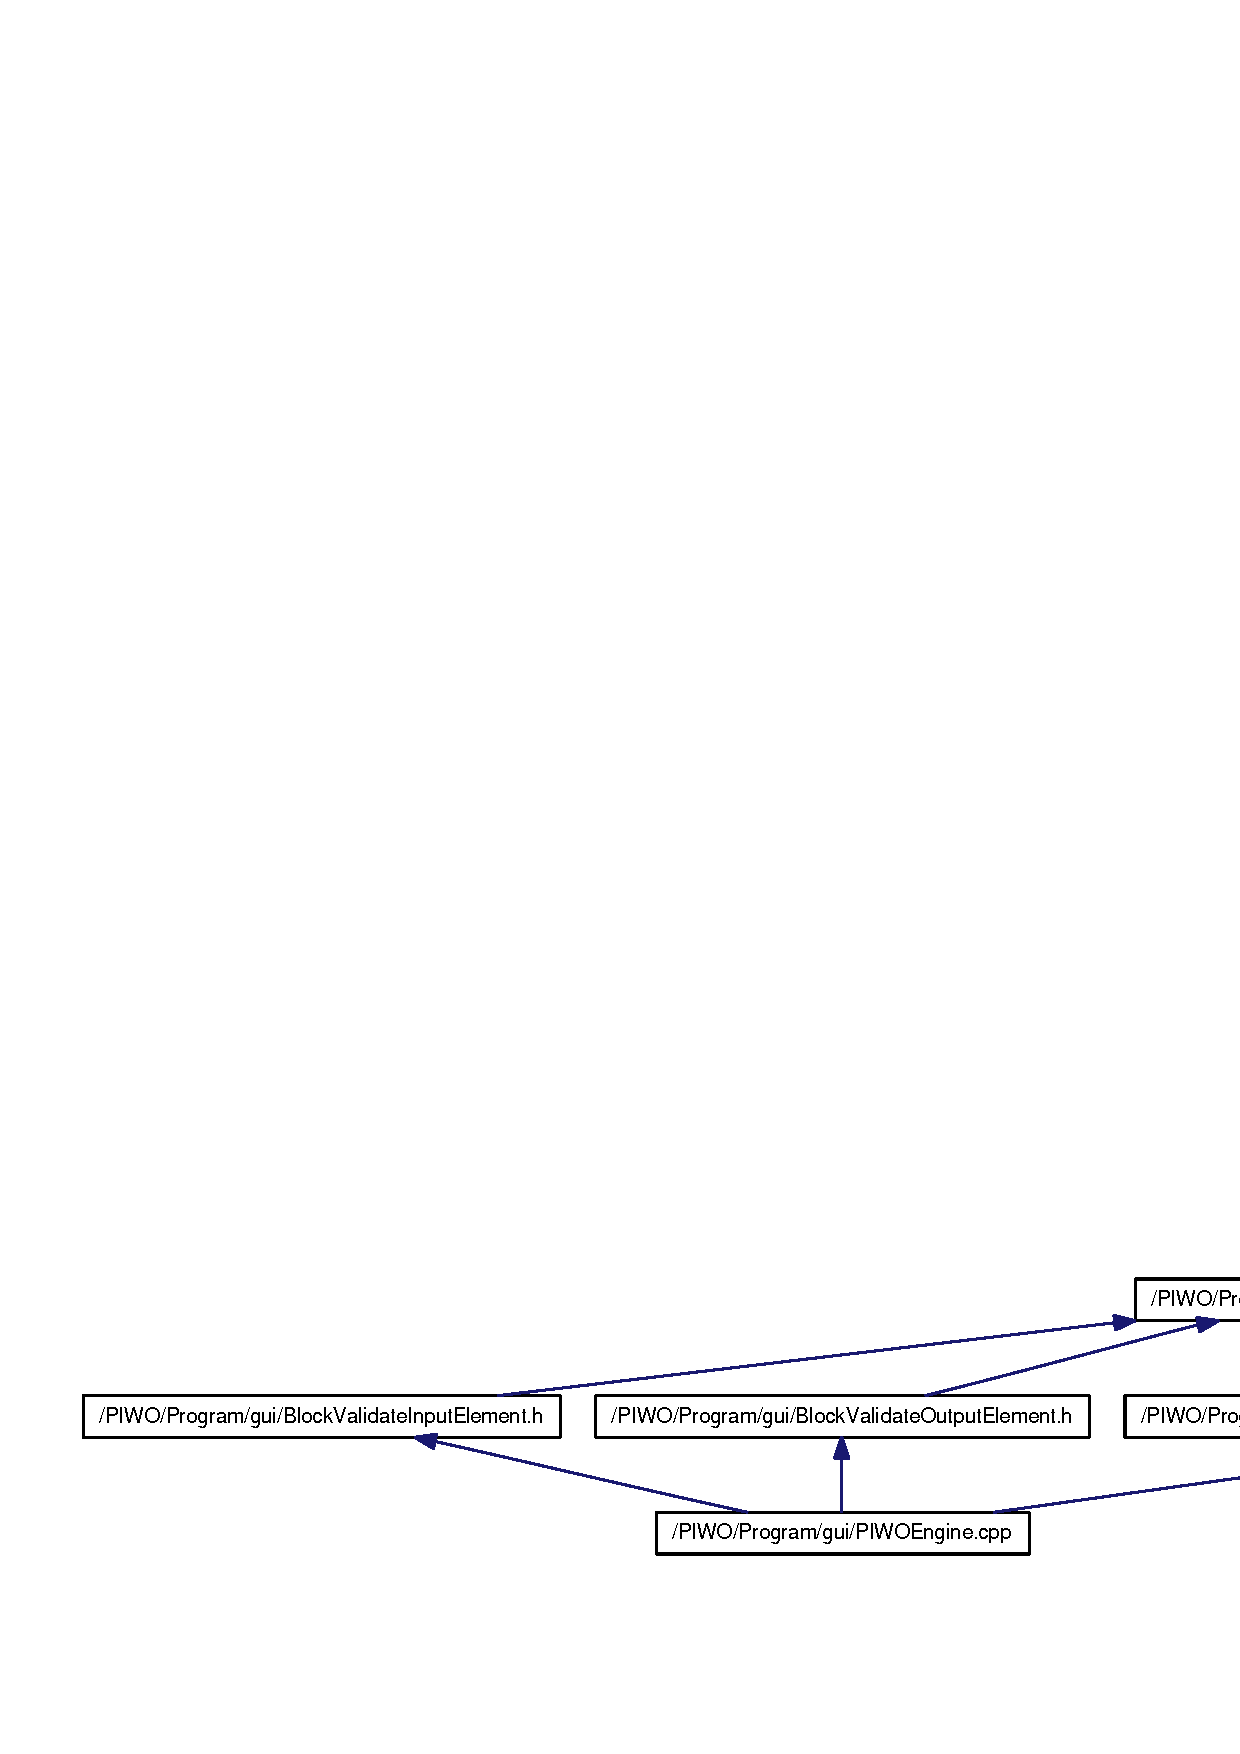
\includegraphics[width=420pt]{Line_8h__dep__incl}
\end{center}
\end{figure}
\subsection*{Classes}
\begin{CompactItemize}
\item 
class \hyperlink{classLine}{Line}
\end{CompactItemize}
\subsection*{Typedefs}
\begin{CompactItemize}
\item 
typedef void(\_\-\_\-closure $\ast$ \hyperlink{Line_8h_9dd4ddd90e5216119027c0f379889e85}{Line\_\-Function} )(TObject $\ast$)
\end{CompactItemize}


\subsection{Typedef Documentation}
\hypertarget{Line_8h_9dd4ddd90e5216119027c0f379889e85}{
\index{Line.h@{Line.h}!Line\_\-Function@{Line\_\-Function}}
\index{Line\_\-Function@{Line\_\-Function}!Line.h@{Line.h}}
\subsubsection[Line\_\-Function]{\setlength{\rightskip}{0pt plus 5cm}typedef void(\_\-\_\-closure $\ast$ {\bf Line\_\-Function})(TObject $\ast$)}}
\label{Line_8h_9dd4ddd90e5216119027c0f379889e85}




Definition at line 7 of file Line.h.